\documentclass[a4paper,11pt]{article}
\usepackage{graphicx}
\usepackage{float}

\begin{document}

% Carátula
\begin{titlepage}
    \centering
    \vspace*{5cm}  
    
    {\Huge\textbf{Trabajo Práctico 2}}\\[1.5cm]
    
    
    % Tabla para alinear nombres sin separación extra
    \begin{tabular}{c}  % 'c' alinea el texto en el centro
        {\Large Juan Manuel Basso}\\
        {\Large Emiliana Verdun}\\
        {\Large Mariana Zunino}
    \end{tabular}

    \vspace{1cm}
    
    {\Large Tecnología Digital VI}\\[0.5cm]
    {\Large Universidad Torcuato Di Tella}\\[0.5cm]
    
    \vfill
    
    {\Large 7 de octubre de 2024}  % Fecha 
\end{titlepage}

% Inicio del contenido del documento
\section{Análisis exploratorio de los datos}

\subsection{Descripción de las variables principales}

El conjunto de datos proporcionado incluye características referidas al usuario como así de la subasta. Las principales variables son:

\begin{itemize}
    \item \textbf{Label}: Es la variable objetivo y representa si un usuario hizo click (1) o no (0) en una publicidad.
    
    \item \textbf{auction\_bidfloor}: Es una variable numérica y puede influir en la propensión de los usuarios a interactuar con anuncios de alto o bajo costo.
    
    \item \textbf{auction\_time}: Representa la hora en que se realizó la subasta. Esta variable es importante ya que el comportamiento del usuario puede variar a lo largo del día y de la semana.
    
    \item Categorías de negocio (\textbf{action\_categorical\_0 a action\_categorical\_7}): Estas variables categóricas identifican diferentes aspectos del negocio y pueden ser claves para identificar patrones de comportamiento en ciertos segmentos de usuarios o tipos de anuncios.
    
    \item \textbf{auction\_age}: Representa la edad del usuario al momento de la subasta, lo que podría estar relacionado con las tendencias de interacción con las publicidades.
\end{itemize}

\subsection{Análisis y Visualización de Patrones}

\subsubsection{Relación entre \textit{auction\_time} y \textit{Label}}

La hora del día en que ocurre la subasta puede influir en el comportamiento del usuario. A continuación, se presenta la distribución de impresiones por hora del día, seguido por la distribución de clicks (\textit{Label = 1}) por hora.

\begin{figure}[H]
    \centering
    \begin{minipage}{0.48\textwidth}
        \centering
        \includegraphics[width=\textwidth]{graficos/impresiones_hora_dia.png}
        \caption{Cantidad de impresiones por hora del día.}
    \end{minipage}
    \hfill
    \begin{minipage}{0.48\textwidth}
        \centering
        \includegraphics[width=\textwidth]{graficos/clicks_hora_dia.png}
        \caption{Cantidad de clicks (\textit{Label = 1}) por hora del día.}
    \end{minipage}
\end{figure}

\subsubsection{Correlación de Pearson entre las Variables y \textit{Label}}

Para identificar las variables más relevantes para predecir los clicks, se calculó el coeficiente de correlación de Pearson entre las principales variables numéricas y la variable \textit{Label}. En el siguiente gráfico se muestran las 8 variables con mayor correlación.

\begin{figure}[H]
    \centering
    \includegraphics[width=0.5\textwidth]{graficos/pearson.png}
    \caption{Correlación de Pearson de las variables con \textit{Label}.}
\end{figure}

\section{Creación de Variables Adicionales}

Durante el análisis, se crearon varias variables adicionales con el fin de mejorar la capacidad predictiva del modelo. A continuación, se describen las principales:

\begin{itemize}
    \item \textbf{Interacción entre \textit{auction\_bidfloor} y \textit{auction\_age}}: Se generó la variable \textit{bidfloor\_age\_interaction}, que representa el producto entre el valor mínimo de oferta en una subasta (\textit{auction\_bidfloor}) y la edad del usuario al momento de la subasta (\textit{auction\_age}). La idea detrás de esta interacción es capturar posibles efectos conjuntos entre el costo de los anuncios y la edad del usuario en la probabilidad de hacer click.

    \item \textbf{Cuadrado de la altura del anuncio (\textit{creative\_height\_squared})}: Se generó una nueva variable a partir de elevar al cuadrado la altura original del anuncio (\textit{creative\_height}). Esto permite capturar posibles relaciones no lineales entre el tamaño del anuncio y la probabilidad de que un usuario haga click.
    
    \item \textbf{Hora del día (\textit{hour})}: A partir de la variable \textit{auction\_time}, que representa el momento exacto en que ocurrió la subasta, se extrajo la hora del día. Esto nos permite analizar patrones de comportamiento de los usuarios en función de las horas del día, ya que la actividad de los usuarios puede variar considerablemente a lo largo del día.
    
    \item \textbf{Día de la semana (\textit{day\_of\_week})}: De forma similar, se generó una variable que indica el día de la semana en que ocurrió la subasta. Esto puede ser útil para identificar patrones semanales en el comportamiento de clicks.
    
    \item \textbf{Indicador de fin de semana (\textit{is\_weekend})}: Esta variable booleana indica si la subasta ocurrió durante el fin de semana. La hipótesis es que el comportamiento de los usuarios podría ser diferente entre los días de semana y los fines de semana.
\end{itemize}

Estas nuevas variables fueron diseñadas para capturar más información sobre el comportamiento de los usuarios y mejorar el rendimiento predictivo del modelo.

\section{Conjunto de Validación}

Para armar el conjunto de validación, se utilizó la técnica de \textit{train-test split}, dividiendo los datos en un 80\% para entrenamiento y un 20\% para validación.

La proporción 80/20 fue seleccionada porque ofrece una cantidad suficiente de datos para entrenar el modelo, al mismo tiempo que permite evaluar su rendimiento en un conjunto de validación no visto durante el entrenamiento.

En resumen, esta estrategia de validación asegura que el modelo se entrene de manera adecuada y se evalúe su rendimiento antes de realizar predicciones sobre el conjunto de prueba final.


\section{Modelos Predictivos y Búsqueda de Hiperparámetros}

En este trabajo se utilizaron dos modelos principales de aprendizaje automático para predecir si un usuario haría click en una publicidad: \textbf{XGBoost} y \textbf{LightGBM}. A continuación, se explica el proceso de optimización de cada modelo y el desempeño obtenido.

\subsection{XGBoost}

El modelo XGBoost se seleccionó debido a su capacidad para manejar grandes volúmenes de datos y su buen rendimiento en problemas de clasificación binaria. Para optimizar los hiperparámetros, se realizó una búsqueda mediante el método de \textit{Randomized Search}, explorando los siguientes parámetros: max_depth, learning_rate, n_estimators, gamma, subsample y colsample_bytree.

Esta búsqueda permitió probar diferentes combinaciones de estos parámetros, y tras múltiples iteraciones, se identificaron los hiperparámetros que ofrecieron el mejor rendimiento para este modelo.

\subsection{LightGBM}

El modelo LightGBM, por su parte, fue seleccionado debido a su eficiencia en términos de tiempo de entrenamiento y su capacidad para manejar grandes conjuntos de datos. A diferencia de XGBoost, en este caso se optó por realizar un ajuste manual de hiperparámetros basado en la experiencia previa y los resultados obtenidos durante el proceso de validación. Entre los parámetros ajustados destacan: n_estimators, max_depth, learning_rate y boosting type.

Este ajuste permitió optimizar el rendimiento del modelo LightGBM de manera eficiente, resultando en una mejor capacidad predictiva en comparación con XGBoost.

\subsubsection{Comparación de Rendimientos}

Tras realizar las pruebas con ambos modelos, \textbf{LightGBM} fue el que obtuvo los mejores resultados en términos de AUC, lo que lo convirtió en el modelo final seleccionado. Aunque XGBoost también mostró un buen rendimiento, LightGBM se destacó por su velocidad y eficiencia en el manejo del conjunto de datos, además este modelo tiene la capacidad de manejar variables categóricas cosa para lo cual xgboost necesita transformaciones, como one-hot encoding, que al ser tan grande el conjunto de datos tardaban demasiado tiempo. 

\section{Importancia de Atributos en el Modelo Final}
    
\begin{figure}[H]
    \centering
    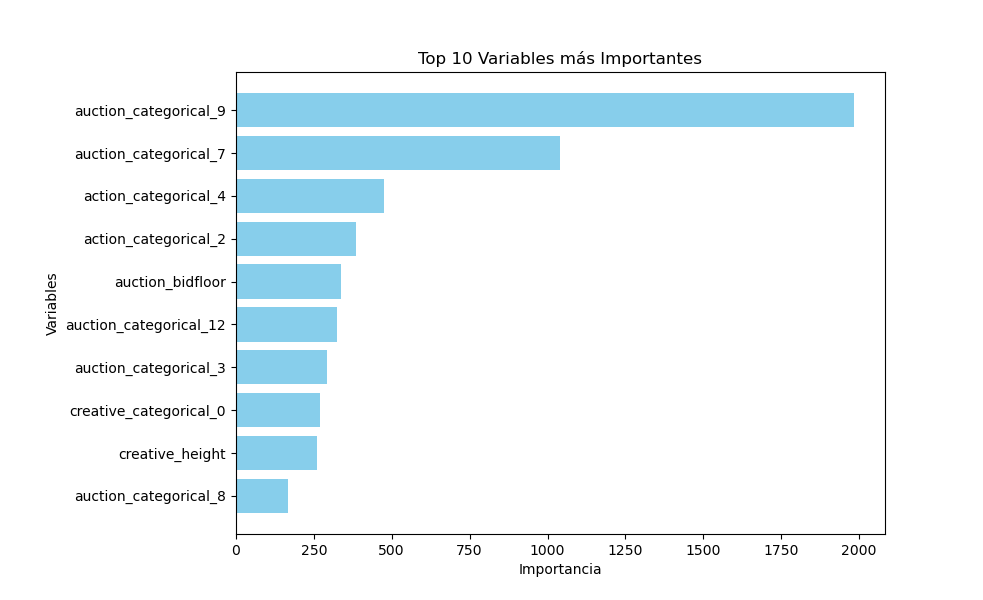
\includegraphics[width=0.5\textwidth]{importancia_modelo.png}
    \caption{Atributos más importantes \textit{Label}.}
\end{figure}

En nuestro modelo final, el que usa LightGBM, se ve que en las variables con más importancia la mayoría son justamente las variables categóricas.



\end{document}

